\documentclass[12pt,a4paper]{article}
\usepackage[utf8]{inputenc}
\usepackage[german]{babel}
\usepackage[T1]{fontenc}
\usepackage{amsmath}
\usepackage{amsfonts}
\usepackage{amssymb}
\usepackage{graphicx}
\usepackage{siunitx}
\usepackage{float}
\usepackage[left=2cm,right=2cm,top=2cm,bottom=2cm]{geometry}
\usepackage{hyperref}
\author{Gerald}


\begin{document}
\sisetup{separate-uncertainty = true}
	\setlength{\parindent}{0pt} 
	\begin{center}
		{\LARGE Versuchsprotokoll}\\
		\begin{large}
			zum Fortgeschrittenenpraktikum im Bachelorstudiengang Physik\\[0.4cm]
			an der RWTH Aachen\\
			II. Physikalisches Institut A\\[5.5cm]
			\Large\textbf{\textsl{Röntgenspektroskopie (T06)}}\\[5.5cm]
			\normalsize\textit{vorgelegt\\von}\\[0.4cm]
			\large{Moritz Berger (355244)\\Gerald Kolter (355005)}\\\textbf{Gruppe 30}\\[2cm]
			\large \textbf{Wintersemester 2017/18}
		\end{large}
	\end{center}
	\newpage
	
	\tableofcontents
	\newpage
	
\section{Hintergund}
Wenn man Materialien mit hochenergetischen Teilchen bestrahlt, so wechelwirken diese folgendermaßen mit den darin enthaltenden Atomen\footnote{Quelle:}:
\begin{enumerate}
\item Bei der Bewegung durch das Material werden die Teilchen abgebremst. Die dabei freiwerdende Energie äußert sich als ein kontinuirliches elektromagnetisches Spektrum, das Bremsstrahlung genannt wird. Die Intensität dieser Strahlung nimmt mit der Masse der abgebremsten Teilchen ab.
\item Die Teilchen geben ihre Energie an ein Elekron im Atom ab, was infolgedessen ionisiert wird. Dadruch wird eine Elektronposition frei und ein höherenergetisches Elektron im Atom kann auf diese Position fallen, wobei ein Röntgenquant abgestrahlt wird. Diesem Übergang kann eine diskrete Energie zugeordent werden. In der Realität äußert er sich wegen Energieunsicherheiten als Gau
\end{enumerate}
Der zweite Effekt hängt direkt von dem Atomaufbau ab, wodurch sich das dadurch ausgestrahlte Spektrum je nach Element unterscheidet. Dadurch kann man die Zusammensetzung eines Materials untersuchen, was in diesem Versuch ausgenutzt wird.
In diesem Versuch wird sowohl ein $\alpha$-Strahler, als auch eine Röntgenquelle als Quelle der hochenergetischen Teilchen benutzt.\\
Ziel ist es, beide Aufbauten mithilfe von mehreren Proben bekannter Zusammensetzung zu kalibrieren, um dann eine Reihe von unbekannten Proben mithilfe ihrer Röntgenpeaks zu untersuchen.
\section{Aufbau}
\subsubsection{$\alpha$-Quelle}
Der erste Aufbau besteht einem X-123 Spektrometer, welches aus einem Halbleiterdetekor der Kennung XR100CR und einem digitalen Pulsprozessor DP5 besteht, der die vom Detektor regristrierten Signale verstärkt und digitalisiert. Der Detektor kann maximal Energien von c.a \SI{60}{keV} aufnehmen, da Teilchen mit größerer Energie den Detektor durchfliegen.\\
Diese Signale werden an einen PC weitergeleitet, wo sie mit dem Programm und der Software ADMCA\footnote{\url{http://amptek.com/products/dpp-mca-display-acquisition-software/}} mithilfe eines Multi-Channel-Analyzers (MCA) nach ihrer Energie auf 496 Kanäle aufgeteilt werden.\\
Zur Kalibration dieser Channels gegen die Energie wird eine variable Röntgenstrahlquelle der Kennung 0317LA benutzt, welche aus einer $^{241}AM$-Quelle besteht, die $\alpha$-Strahlung auf ein durch eine Drehscheibe variables Target strahlt. Diese Quelle wird direkt vor den Detektor gestellt.\\
Zur Aufnahme von unbekannten Proben wird eine $^{241}AM$-Quelle der Kennummer Z3715 benutzt, welche in eine Bleibefestigung eingelassen wird.
\subsubsection{Röntgenquelle}
Bei den Messungen mit der Röntgenquelle wird ein X-123 Spektrometer der gleichen Bauart wie oben beschrieben verwendet. Die Röntgenquelle hat die Kennnummer BJ8288.
\section{Durchführung}
\subsubsection{$\alpha$-Quelle}
Als erstes muss über eine Kalibration den Channels eine Energie zugeordent werden.\\
Die dafür benutzte variable Röntgenstrahlquelle besitzt 6 Targets aus verschiedenen Materialien: Cu, Rb, Mo, Ag, Ba und Tb.\\
Bevor die Messungen gestartet werden können, muss an dem benutzten Programm der richtige Messbereich eingestellt werden. Dies geschieht an dem Tb Spektrum, da diese Probe Röntgenstrahlung mit der größten Energie aussendet, welche außerdem knapp unterhalb der maximal messbaren Energie liegt.\\
Dazu wird in den Programmeinstellungen der Verstärkungsfaktor so eingestellt, dass die Linie mit der größten Energie möglichst weit rechts im sichtbaren Spektrum liegt.\\
Außerdem kann über den Reiter "shaping" eine "Pile-up Rejection"(PUR) und eine "Rise Time Discrimination"(RTD) zugeschaltet werden. Bei einer Schnellauswertung haben diese Einstellungen aber keinen nennenswerten Unterschied gemacht, weswegen sie für die Messungen deaktiviert wurden.\\
Alle Einstellung sind in Tabelle \ref{tab:alpha_Einstellungen} aufgelistet.\\
\\
Nun wird für jede der sechs Proben über \SI{15}{min} das Spektrum aufgenommen.\\
Danach werden für eine Edelstahlplatte ebenfalls über \SI{15}{min} die Spektren aufgenommen.\\
Außerdem wird noch eine Leermessung über diesen Zeitraum aufgenommen. Dazu wird ein Stück Papier in die Probenkammer gelegt, damit der Effekt einer Probe simuliert werden kann.\\
Für beide Messungen wird die $\alpha$-Quelle in eine massive Halterung gelegt, welche einen Raum für Proben besitzt. Die Strahlung wird dabei von der Probe zum Zahlrohr hin reflektiert.
\begin{table}
\centering
\begin{tabular}{|c|c|}
\hline 
Einstellung & Wert \\ 
\hline 
Gain(coarse) & 2.1x \\ 
\hline 
Gain(fine) & 0.95 \\ 
\hline 
RTD & aus \\ 
\hline 
PUR & aus \\ 
\hline 
Messzeit & 15 min \\ 
\hline 
\end{tabular} 
\caption{Einstellungen für die Messungen mit der $\alpha$-Quelle.}
\label{tab:alpha_Einstellungen}
\end{table}
\subsection{Röntgenquelle}

\section{Ergebnisse $\alpha$-Quelle}
\subsection{Kalibration}

\begin{figure}
\centering
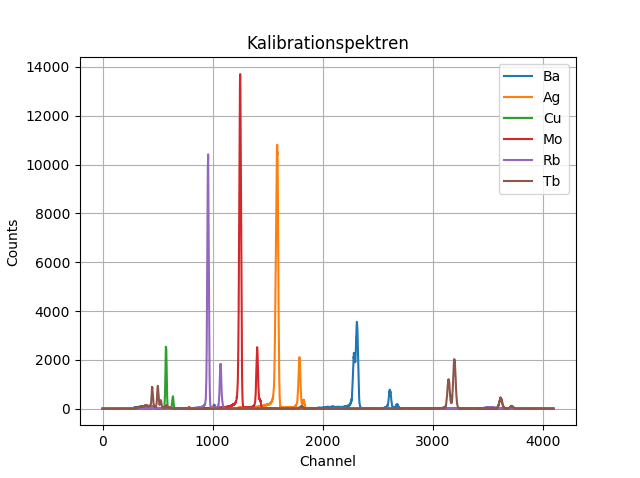
\includegraphics[scale=0.9]{Bilder/alpha/kal_alles.png}
\caption{Alle für dei Kalibration aufgenommenen Spektren.}
\label{fig:kal_alles}
\end{figure}

Die Spektren der sechs Proben sind in Abbildung \ref{fig:kal_alles} gezeigt.\\
Da das Rauschen in den Daten nicht sehr groß ist wird auf einen Frequenzcutoff verzichtet.\\
Für alle Spektren ist der $K_{\alpha}$ und der $K_{\beta}$ Peak zu sehen.
Nun wird an diese Peaks ein Gaussfit angepasst. Dies ist in Abbildung \ref{fig:kal_fits} beispielhaft gezeigt. Die restlichen Anpassungen befinden sich im Anhang.\\
Bei Peaks mit höheren Energien wird die Feinstrukturaufspaltung immer sichtbarer, bis man die Linien eindeutig trennen kann, wie in Abbildung \ref{fig:kal_fein} anhand des Barium $K_{\alpha}$-Peaks zu sehen. Da sich die beiden Linien aber immernoch überlagern, ist die sichtbare Position der Peaks leicht versetzt. Um die wahre Position bestimmen zu können, wird eine doppelte Gaußfunktion angefittet, die die Positionen beider Peaks bestimmt.\\
Die Feinstruktur tritt natürlich auch bei den niedrigenergetischen Peaks auf. Hier äußert sie sich dadurch, dass der Peak nicht exakt gaussförmig ist,sondern eine unterschiedliche Flankensteigung auf beiden Seiten hat. Dadurch verschiebt sich die Position leicht, wenn man den Anpassungsbereich vergrößert.\\
Um den Fehler auf die Position besser abschätzen zu können, wird deswegen einmal ein kleiner und einmal ein großer Bereich an die Peaks angepasst. Der Unterschied in der Peakposition wird als Fehler angenommen, solange dieser größer als der Fitfehler ist.\\
Als Peakposition wird immer die mit dem kleineren Fehler genommen, da dise den jeweiligen Peak genauer beschreibt.\\
\\
An den so bestimmten Peaks wird nun eine Energiekalibration durchgeführt. Dazu wird den Peaks eine Energie zugeordnet, die den Literaturwerten entnommen wurde, welche in Tabelle \ref{tab:alpha_lit} aufgelistet sind. Falls in einem Peak mehrere Literaturwerte liegen, so wird der Wert genommen, dessen Peak die höhere Intensität hat. Dies ist immer $K_{\alpha_1}$ und $K_{\beta_{1}}$.\\
Nun wird eine lineare Regression durchgeführt, die den Channels eine Energie zuweist. Dies ist in Abbildung \ref{fig:kal_linreg} zu sehen. Daraus ergibt sich eine Kalibrationsgrade von
\begin{equation}
E = (0.013904\pm0.000004)\cdot CH + (0.060\pm0.010)
\end{equation}
wobei die Energie in keV angegeben wird (CH steht für Channel). Der Fehler auf die Energien wird dann folgendermaßen errechnet:
\begin{equation}
\sigma_E = \sqrt{\sigma_b^2+(\sigma_a\cdot CH)^2}
\end{equation}
wobei b der Achsenabschnitt und a die Steigung ist.

\begin{table}
\centering
\begin{tabular}{|c|c|c|c|c|}
\hline 
Probe & $K_{\alpha_1}$ & $K_{\alpha_2}$ & $K_{\beta_2}$ & $K_{\beta_{1/3}}$ \\ 
\hline 
Cu & $576.8\pm0.2$ & - & -& $638.5\pm0.6$\\ 
\hline 
Rb & $958.1\pm0.1$ & - & -& $1071.5\pm0.4$\\ 
\hline 
Mo & $1249.8\pm1.5$ & - & $1430.0\pm0.9$ & $1404.1\pm0.4$ \\ 
\hline 
Ag & $1588.7\pm1.0$ & - & $1825.1\pm0.2$ & $1787.5\pm0.3$ \\ 
\hline 
Ba & $2310.1\pm0.8$ & $2282.8\pm0.9$ & $2674.6\pm0.2$ & $2609.4\pm0.3$ \\ 
\hline 
Tb & $3195.4\pm0.2$ & $3152.7\pm0.1$ & $3715.4\pm0.4$ & $3616.1\pm0.4$ \\ 
\hline 
\end{tabular} 
\caption{Peakpositionen in den Channels der abgelesenen Peaks. Falls keine Feinstrukturaufspaltung ermittelt werden konnte, wurd angenommen, dass der Peak immer der mit der größeren Intensität ist.}
\label{tab:alpha_kal}
\end{table}

\begin{table}
\centering
\begin{tabular}{|c|c|c|c|c|c|}
\hline 
Probe & $K_{\alpha_1}$ & $K_{\alpha_2}$ & $K_{\beta_2}$ & $K_{\beta_{1}}$ & ($K_{\beta_{3}}$) \\ 
\hline 
Cu & 8,047.8 & 8,027.8 & - & 8,905.3 & 8,905.3\\ 
\hline 
Rb & 13,395.3 & 13,335.8  & 15,185 & 14,961.3 & 14,951.7\\ 
\hline 
Mo & 17,479.3 & 17,374.3 & 19,965.2  & 19,608.3 & 19,590.3\\ 
\hline 
Ag & 22,162.9 & 21,990.3 & 25,456.4 & 24,942.4 & 24,911.5\\ 
\hline 
Ba & 32,193.6 & 31,817.1 & 37,257 & 36,378.2 & 36,304.0\\ 
\hline 
Tb & 44,481.6 & 43,744.1 & 51,698 & 50,382 & 50,229\\ 
\hline 
\end{tabular} 
\caption[test]{Literaturwerte\footnotemark für die Peakpositionen. Alle Angaben sind in eV, wobei nach der 1000eV stelle ein Komma steht.}
\label{tab:alpha_lit}
\end{table}
\footnotetext{Quelle: \url{http://xdb.lbl.gov/Section1/Table_1-3.pdf}}

\begin{figure}
\centering
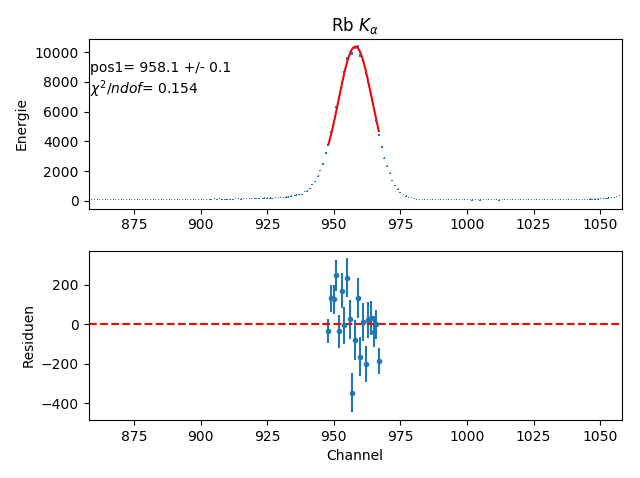
\includegraphics[scale=0.8]{Bilder/alpha/rb_alpha_1.png}
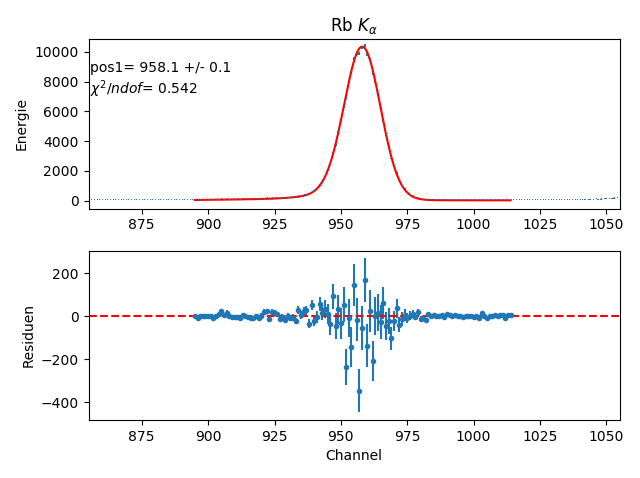
\includegraphics[scale=0.8]{Bilder/alpha/rb_alpha_2.png}
\caption{Beispiel für den Gaußfit anhand des $K_{\alpha}$ Peaks von Rubidium. In diesem Peak liegen $K_{\alpha_1}$ und $K_{\alpha_1}$ sehr eng nebeneinander, weswegen der Peak gaussförmig ist und sich die Position bei Vergrößerung kaum verändert}
\label{fig:kal_fits}
\end{figure}

\begin{figure}
\centering
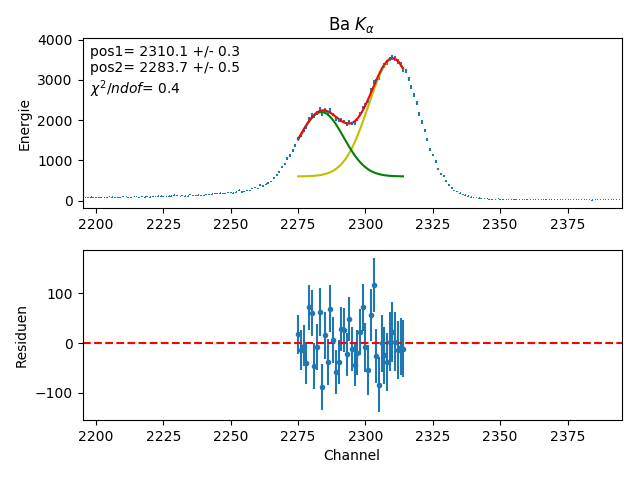
\includegraphics[scale=0.8]{Bilder/alpha/ba_alpha_1.png}
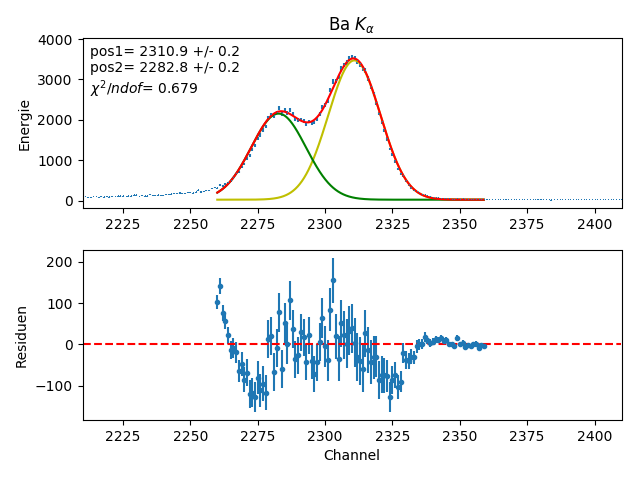
\includegraphics[scale=0.8]{Bilder/alpha/ba_alpha_2.png}
\caption{Doppelter Gaussfit (in rot) an sich überlappende Peaks. Bei der Änderung des Fitbereiches ändert sich auch die Positionder Peaks. Es sind außerdem die beiden einzelnen Peaks eingezeichnet (gelb und grün).}
\label{fig:kal_fein}
\end{figure}

\begin{figure}
\centering
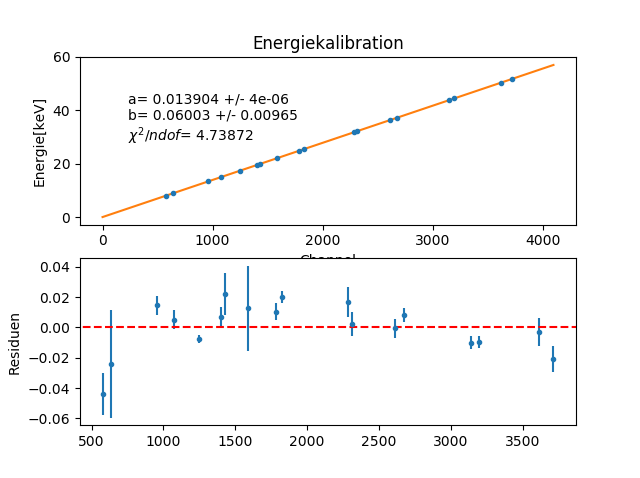
\includegraphics[scale=0.8]{Bilder/alpha/kal.png}
\caption{Lineare Regression an den Channelpositionen und der zugewiesenen Energie. Der jeweilige Fehler der Datenpunkte ist der Maximalfehler aus Fit und Fitvariation.}
\label{fig:kal_linreg}
\end{figure}


\newpage
\subsection{Auswertung unbekannter Proben}
\begin{figure}
\centering
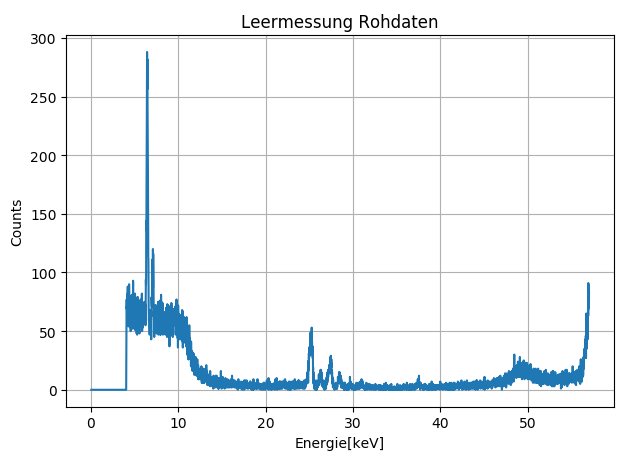
\includegraphics[scale=0.8]{Bilder/alpha_spektren/leer_roh.png}
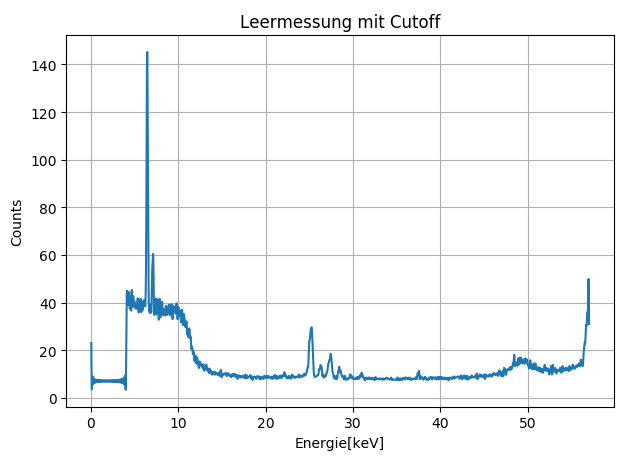
\includegraphics[scale=0.8]{Bilder/alpha_spektren/leer_cut.png}
\caption{Leermessung. \textbf{Oben:} Rohdaten, \textbf{unten:} Daten nach Bearbeitung mit dem Tiefpassfilter.}
\label{fig:a_prob_leer}
\end{figure}

\begin{figure}
\centering
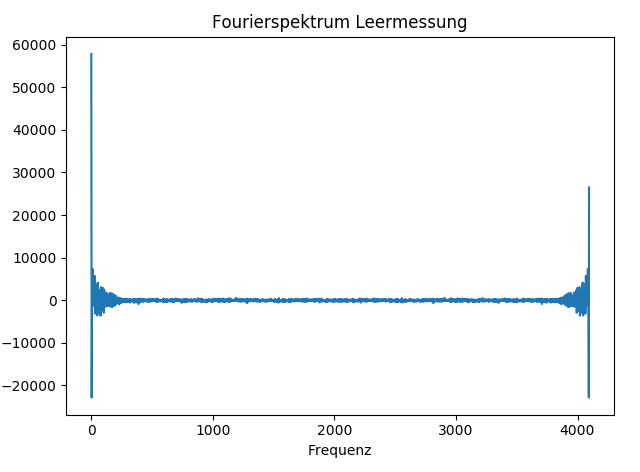
\includegraphics[scale=0.8]{Bilder/alpha_spektren/leer_fourier.png}
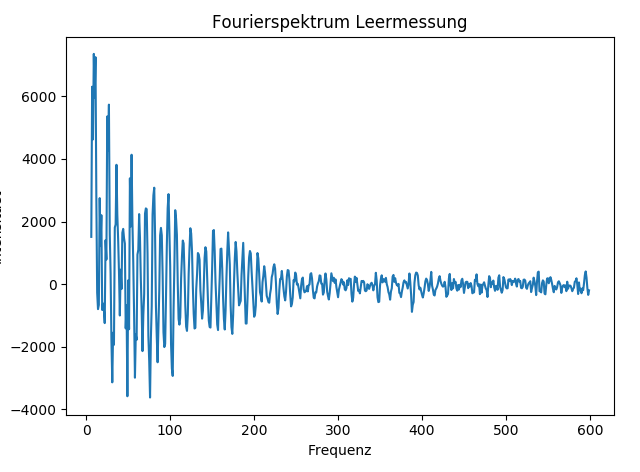
\includegraphics[scale=0.8]{Bilder/alpha_spektren/leer_fourier_2.png}
\caption{Frequenzspektrum der Leermessung und hereingezoomter Bereich. Die cutofffrequenz wurde mit 300 festgelegt.}
\label{fig:a_prob_four}
\end{figure}

\begin{figure}
\centering
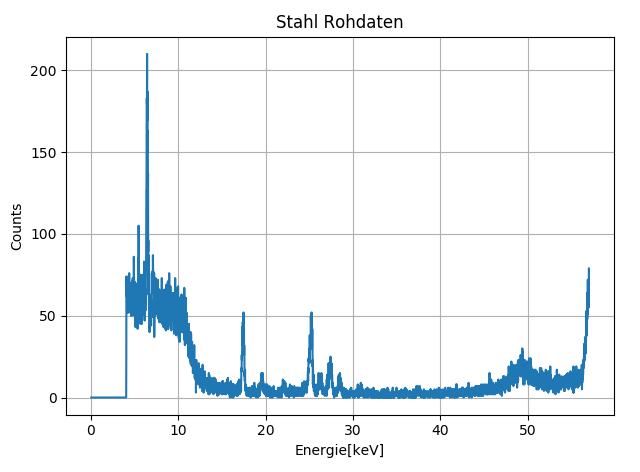
\includegraphics[scale=0.8]{Bilder/alpha_spektren/stahl_roh.png}
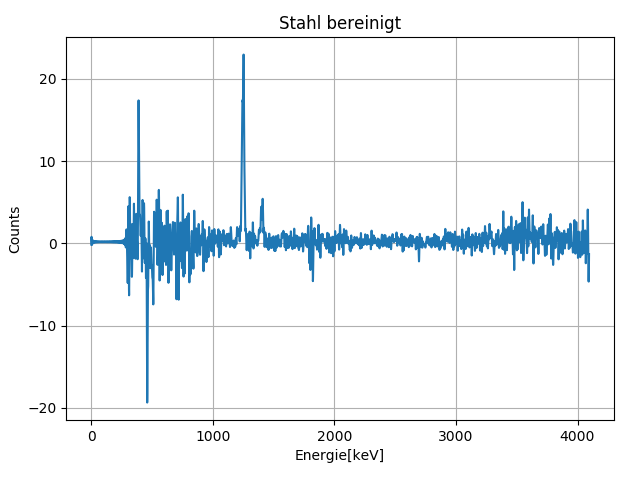
\includegraphics[scale=0.8]{Bilder/alpha_spektren/stahl_cut.png}
\caption{Spektrum des Stahls. \textbf{Oben:} Rohdaten, \textbf{unten:} Daten mit Tiefpassfilter bereinigt und Leermessung abgezogen.}
\label{fig:a_prop_stahl}
\end{figure}

Mit der Energiekalibration können nun die unbekannten Proben ausgewertet werden. Dazu muss zuerst eine Leermessung durchgeführt werden, um die Hintergrundstrahlung herausfiltern zu können. Diese ist in Abbildung \ref{fig:a_prob_leer} gezeigt. Um Peaks besser erkennen zu können und das Rauschen zu verringern wird ein Tiefpassfilter auf die Daten angewendet. Dazu werden die Daten fouriertransformiert, was in Abbildung \ref{fig:a_prob_four} gezeigt ist. Die Cutoff-Frequenz wurde auf 300 festgelegt, dass heißt, dass alle Frequenzen auf null gesetzt werden, die größer als 300 sind. Das übrige Fourierspektrum wird dann zurücktransformiert. Das Spektrum mit Tiefpassfilter ist jeweils unter den Rohdaten mit angegeben.\\
\\
An die sichtbaren Peaks der Leermessung ohne Tiefpassfilter werden wieder Gausskurven angefittet, um deren Lage zu bestimmen. Die Ergebnisse sind in Tabelle \ref{tab:a_peaks_leer} aufgelsitet. Alle Anpassungen befinden sich im Anhang.\\
Der Fehler wird wieder durch verschieben der Anpassung bestimmt. Außerdem planzt sich ein systematischer Fehler aus der Kalibration fort, welcher aber nicht mit in die Anpassung einfließt.\\
Bei machnen Peaks kann es sein, dass deren Höhe zu klein ist. Dann funktioniert der Fit nicht fernünftig. Es wird dann stattdessen ein Fit an die Daten mit Tiefpassfilter angepasst.\\
\\
Danach wird die gleiche Methode auf die Messung des rostfreihen Stahles angewandt. 
Von dessen Rohdaten wird aber zuerst die Leermessung abgezogen. 
Auch hier wird ein Tiefpassfilter auf die Daten angewendet.\\
Das Spektrum ist in Abbildung \ref{fig:a_prop_stahl} dargestellt, die bestimmten PEaks in Tabelle \ref{tab:a_peaks_stahl}.

\subsubsection{Vergleich mit Erwartung}
Im Spektrum der Stahlplatte konnte eindeutig Molybdän identifiziert werden. Dieses wird in Stahl zur Härtung benutzt\footnote{\url{http://www.chemie.de/lexikon/Molybdän.html}}. der 5.477keV Peak konnte nicht eindeutig identifiziert werden. Da Chrom aber oft in Legierungen verwendet wird\footnote{\url{http://www.seilnacht.com/Lexikon/24Chrom.htm}}, gehört dieser Peak wahrscheinlich zu diesem Stoff.\\
\\
In der Leermessung wurde im Grunde das Spektrum des Probenhalterblockes aufgenommen. Dieser beinhaltetet offensichtlich Zinn  und sehr wahrscheinlich Eisen, da beiden Elementen zwei Linien zugeordent werden konnten. 
Außerdem wurde Tellur (Te)\footnote{\url{http://www.rsc.org/periodic-table/element/52/tellurium}} und Antimon (Sb) \footnote{\url{http://www.seilnacht.com/Lexikon/51Antim.htm}} gefunden. Diese Stoffe werden auch in Legierungen verwendet, es kann also sein, dass sie bei der Stahlplattenmessung nicht nur Hintergrundrauschen waren.\\
Das gleiche gilt für Eisen, was ein Hauptbestandteil von Stahl ist\footnote{\url{https://de.wikipedia.org/wiki/Rostfreier_Stahl}}.

\begin{table}
\center
\begin{tabular}{|c|c|c|c|c|}
\hline 
Peakpos.[keV] & Stoff & Linie & Literaturwert[keV] & Anmerkung \\
\hline 
$25.17\pm 0.01\pm 0.01$& $^{50}Sn$ & $K_{\alpha_{1/2}}$ & $25.04-25.27$ & \\ 
\hline 
$26.29\pm 0.03\pm 0.01$ & $^{51}Sb$ & $K_{\alpha_{1/2}}$ & $26.11-26.36$ & \\ 
\hline 
$27.37\pm 0.03\pm 0.01$ & $^{52}Te$ & $K_{\alpha_{1/2}}$ & $27.20-27.47$ & \\ 
 & $^{49}In$ & $K_{\beta_{1/3}}$ & $27.237-27.276$ & unwahrsch.: $K_{\alpha}\approx 24.2keV$ nicht sichtbar\\ 
\hline 
$28.42\pm 0.02\pm 0.01$ & $^{50}Sn$ & $K_{\beta_{1/3}}$ & $28.44-28.48$ &\\ 
\hline 
$6.456\pm 0.001\pm 0.010$ & $^{26}Fe$ & $K_{\alpha_{1/2}}$ & $6.439-6.404$ &\\ 
& $^{63}Eu$ & $L_{\beta_{2}}$ & $6.456$ & unwahrsch.: $K_{\alpha/\beta}\approx 40keV$ nicht sichtbar\\
& $^{25}Mn$ & $K_{\beta_{1/3}}$ & $6.490$ & unwahrsch.: $K_{\alpha}\approx 5.8keV$ nicht sichtbar\\
\hline 
$7.096\pm 0.001\pm 0.010$ & $^{26}Fe$ & $K_{\beta_{1/3}}$ & $7.058$ & \\ 
& $^{64}Gd$ & $L_{\beta_{2}}$ & $7.103$ & unwahrsch.:$K_{\alpha/\beta}\approx 43keV$ nicht sichtbar\\
\hline 
\end{tabular} 
\caption{Peaks in der Leermessung}
\label{tab:a_peaks_leer}
\end{table}

\begin{table}
\center
\begin{tabular}{|c|c|c|c|c|}
\hline 
Peakpos.[keV] & Stoff & Linie & Literaturwert[keV] & Anmerkung \\
\hline 
$5.477\pm 0.05\pm 0.01$& $^{24}Cr$ & $K_{\alpha_{1}}$ & $5.415$ & \\ 
& $^{23}V$ & $K_{\beta_{1/3}}$ & $5.427$ & unwahrsch.: $K_{\alpha}\approx 4.9keV$ nicht sichtbar\\ 
& $^{61}Pm$ & $L_{\alpha_{1}}$ & $5.432$ & unwahrsch.: $K_{\alpha}\approx 39keV$ nicht sichtbar\\ 
& $^{59}Pr$ & $L_{\beta_{1}}$ & $5.488$ & unwahrsch.: $K_{\alpha}\approx 36keV$ nicht sichtbar\\ 
\hline 
$17.425\pm 0.04\pm 0.01$ & $^{42}Mo$ & $K_{\alpha_{1/2}}$ & $17.374-17.479$ & \\ 
\hline 
$19.57\pm 0.03\pm 0.01$ & $^{42}Mo$ & $K_{\beta_{1/3}}$ & $19.59-19.61$ & \\
 \hline 
\end{tabular} 
\caption{Peaks in der Messung des Stahls}
\label{tab:a_peaks_stahl}
\end{table}

\subsection{Energieauflösung}
\section{Ergebnisse Röntgenquelle}
\subsection{Kalibration}

\subsection{Auswertung unbekannter Proben}
Die Proben mit der Röntgenquelle werden genau so ausgewertet, wie die der $\alpha$-Quelle. Allerdings ist es hier nicht nötig, einen Tiefpassfilter anzuwenden, da das Ruaschen gegenüber der Peakhöhe relativ klein ist.\\
Alle Spektren werden von der Untergrundmessung bereinigt.\\
\\
Die Literaturwerte stammen weiterhin von \url{http://xdb.lbl.gov/Section1/Table_1-3.pdf}.

\newpage
\subsubsection{rostfreier Stahl}
\begin{figure}[H]
\centering
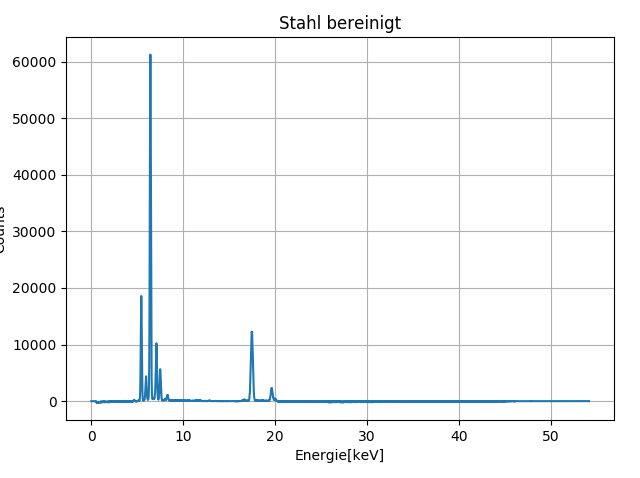
\includegraphics[scale=1]{Bilder/roentgen_spektren/stahl_0.png}
\caption{Von der Leermessung bereinigtes Spektrum des \textbf{Stahles}.}
\label{fig:prop_stahl}
\end{figure}

\begin{table}[H]
\center
\begin{tabular}{|c|c|c|c|c|}
\hline 
Peakpos.[keV] & Stoff & Linie & Literaturwert[keV] & Anmerkung \\
\hline 
$5.423 \pm 0.003 \pm 0.006$& $^{24}Cr$ & $K_{\alpha_{1/2}}$ & $5,405-5,414$ & \\
\hline 
$5.941 \pm 0.002 \pm 0.006$ & $^{24}Cr$ & $K_{\beta_{1/3}}$ & $5,946$ & \\
\hline 
$6.409 \pm 0.001 \pm 0.006$ & $^{26}Fe$ & $K_{\alpha_{1/2}}$ & $6,390-6,403$ & \\
\hline
$7.045 \pm 0.002 \pm 0.006$ & $^{26}Fe$ & $K_{\beta_{1/3}}$ & $7,058$ & \\
\hline
$7.481 \pm 0.001 \pm 0.006$ & $^{28}Ni$ & $K_{\alpha_{1/2}}$ & $7,460-7,478$ & \\
\hline
$8.264 \pm 0.016 \pm 0.006$ & $^{28}Ni$ & $K_{\beta_{1/3}}$ & $8,264$ & \\
\hline
$17.462 \pm 0.004 \pm 0.008$ & $^{42}Mo$ & $K_{\alpha_{1/2}}$ & $17,374-17,479$ & \\
\hline
$19.622 \pm 0.005 \pm 0.008$ & $^{42}Mo$ & $K_{\beta_{1/3}}$ & $19,590-19,608$ & \\
\hline
\end{tabular} 
\caption{Peaks in der Messung des Stahl}
\label{prob_stahl}
\end{table}

\newpage
\subsubsection{Blei}
\begin{figure}[H]
\centering
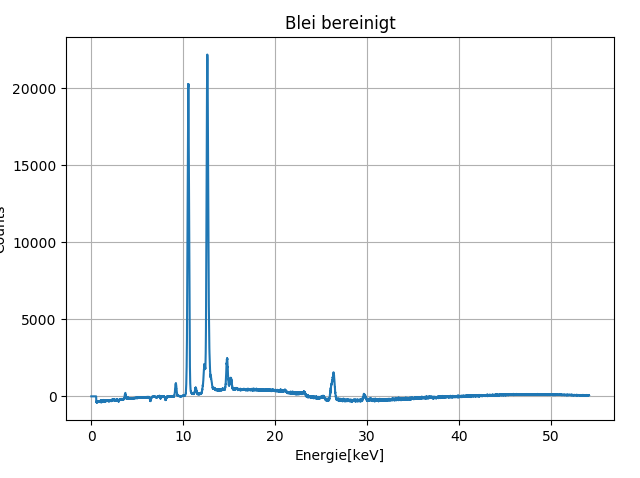
\includegraphics[scale=1]{Bilder/roentgen_spektren/blei_0.png}
\caption{Von der Leermessung bereinigtes Spektrum des \textbf{Bleiblockes}.}
\label{fig:prop_blei}
\end{figure}

\begin{table}[H]
\center
\begin{tabular}{|c|c|c|c|c|}
\hline 
Peakpos.[keV] & Stoff & Linie & Literaturwert[keV] & Anmerkung \\
\hline 
$3.674 \pm 0.0 \pm 0.006$& $^{20}Ca$ & $K_{\alpha_{1/2}}$ & $3,688-3,691$ & Hintergrundstahlung\\
\hline 
$9.183 \pm 0.002 \pm 0.007$ & $^{82}Pb$ & $L_{1}$ & $9,184$ & \\ 
\hline 
$10.54 \pm 0.004 \pm 0.007$ & $^{82}Pb$ & $L_{\alpha_{1/2}}$ & $10,449-10,551$ & \\
\hline
$12.614 \pm 0.0 \pm 0.007$ & $^{82}Pb$ & $L_{\beta_{1/2}}$ & $12,613-12,622$ & \\
\hline
$14.760 \pm 0.003 \pm 0.007$ & $^{82}Pb$ & $L_{\gamma_{1}}$ & $14,764$ & \\
\hline
$15.157 \pm 0.01 \pm 0.007$ & $^{37}Rb$ & $K_{\beta_{1/2}}$ & $14,961-15,185$ & \\
\hline
$26.314 \pm 0.047 \pm 0.01$ & $^{51}Sb$ & $K_{\alpha_{1/2}}$ & $26,110-26,359$ & \\
\hline
$29.717 \pm 0.003 \pm 0.01$ & $^{51}Sb$ & $K_{\beta_{1/3}}$ & $29,679-29,725$ & \\
\hline
\end{tabular} 
\caption{Peaks in der Messung des Bleiblockes}
\label{prop_blei}
\end{table}
\newpage
\subsubsection{Chip}
\begin{figure}[H]
\centering
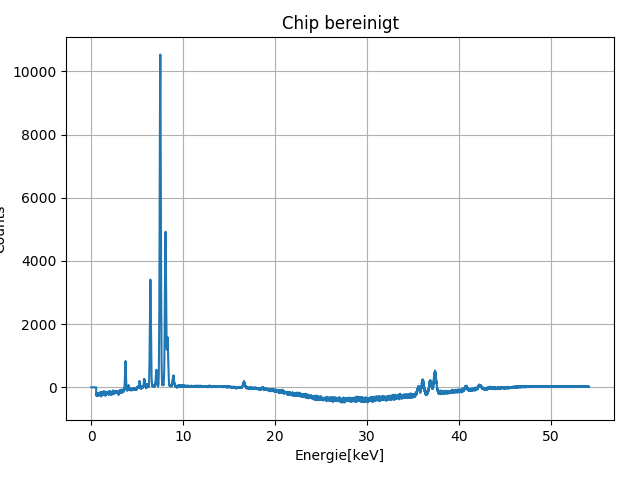
\includegraphics[scale=1]{Bilder/roentgen_spektren/chip_0.png}
\caption{Von der Leermessung bereinigtes Spektrum des \textbf{Computerchips}.}
\label{fig:prop_chip}
\end{figure}

\begin{table}[H]
\center
\begin{tabular}{|c|c|c|c|c|}
\hline 
Peakpos.[keV] & Stoff & Linie & Literaturwert[keV] & Anmerkung \\
\hline 
$3.696 \pm 0.002 \pm 0.006$& $^{20}Ca$ & $K_{\alpha_{1/2}}$ & $3,688-3,691$ & Hintergrundstrahlung\\
\hline 
$6.401 \pm 0.002 \pm 0.006$ & $^{26}Fe$ & $K_{\alpha_{1/2}}$ & $6,390-6,403$ & \\ 
\hline 
$8.409 \pm 0.006 \pm 0.006$ & $^{70}Yb$ & $L_{\beta_{1/2}}$ & $8,401$ & \\
& $^{74}W$ & $L_{\alpha_{1}}$ & $8,397$ & besser, da mehrere Linien gefunden\\
\hline
$9.688 \pm 0.002 \pm 0.007$ & $^{79}Au$ & $L_{\alpha_{1}}$ & $9,713$ & \\
& $^{74}W$ & $L_{\beta_{1}}$ & $9,672$ & besser, da mehrere Linien gefunden\\
\hline
$11.921 \pm 0.003 \pm 0.007$ & $^{80}Hg$ & $L_{\beta_{2}}$ & $11,924$ & \\
& $^{35}Br$ & $K_{\alpha_{1/2}}$ & $11,877-11,924$ & \\
\hline
$12.638 \pm 0.006 \pm 0.007$ & $^{36}Kr$ & $K_{\alpha_{1/2}}$ & $12,598-12,649$ & \\
& $^{82}Pb$ & $L_{\beta_{1/2}}$ & $12,613-12,622$ & \\
\hline
$13.304 \pm 0.001 \pm 0.007$ & $^{35}Br$ & $K_{\beta_{1/3}}$ & $13,284-13,291$ & \\
\hline
$17.464 \pm 0.004 \pm 0.008$ & $^{42}Mo$ & $K_{\alpha_{1/2}}$ & $17,374-17,479$ & \\
\hline
$19.629 \pm 0.011 \pm 0.008$ & $^{42}Mo$ & $K_{\beta_{1/2/3}}$ & $19,590-19,965$ & \\
\hline
$25.239 \pm 0.03 \pm 0.009$ & $^{50}Sn$ & $K_{\alpha_{1/2}}$ & $25,044-25,271$ & \\
\hline
$28.511 \pm 0.003 \pm 0.01$ & $^{50}Sn$ & $K_{\beta_{1/3}}$ & $28,444-28,486$ & besser,da mehrere Linien gefunden\\
& $^{53}I$ & $K_{\alpha_{1/2}}$ & $28,317-28,612$ & \\
\hline
\end{tabular} 
\caption{Peaks in der Messung des Computerchips}
\label{prop_chip}
\end{table}

\subsubsection{Magnet}

\begin{figure}[H]
\centering
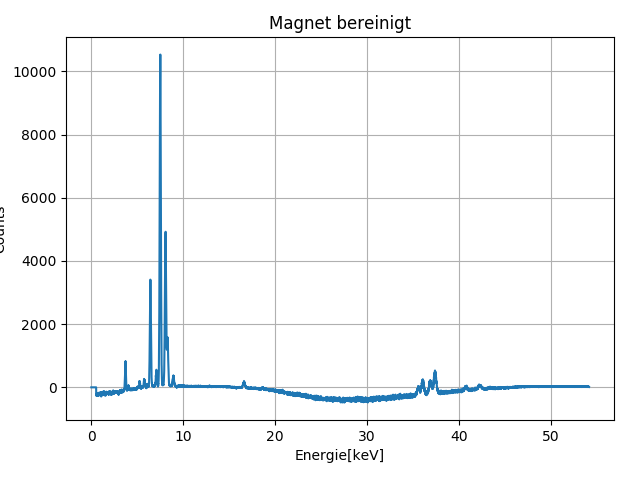
\includegraphics[scale=0.49]{Bilder/roentgen_spektren/magnet_0.png}
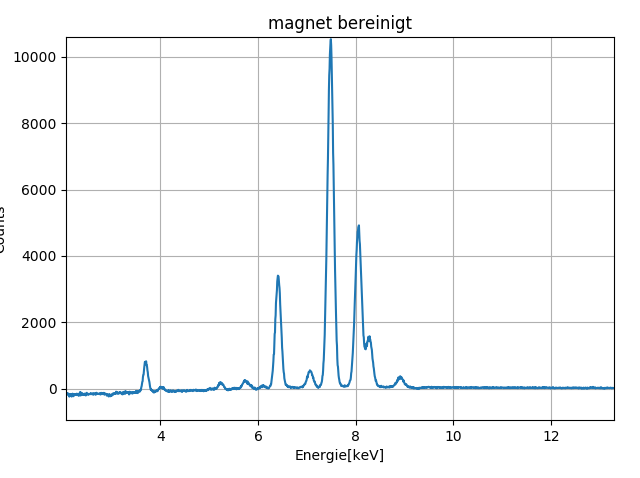
\includegraphics[scale=0.49]{Bilder/roentgen_spektren/magnet_1.png}
\caption{Von der Leermessung bereinigtes Spektrum des \textbf{Magnetes} und zoom in den engen Bereich bei  5-10keV.}
\label{fig:prop_magnet}
\end{figure}

\begin{table}[H]
\center
\begin{tabular}{|c|c|c|c|c|}
\hline 
Peakpos.[keV] & Stoff & Linie & Literaturwert[keV] & Anmerkung \\
\hline 
$3.7 \pm 0.002 \pm 0.006$& $^{20}Ca$ & $K_{\alpha_{1/2}}$ & $3,688-3,691$ & Hintergrundstahlung\\
\hline 
$5.236 \pm 0.001 \pm 0.006$ & $^{60}Nd$ & $L_{\alpha_{1/2}}$ & $5,207-5,230$ & \\ 
\hline 
$5.747 \pm 0.017 \pm 0.006$ & $^{66}Dy$ & $L_{1}$ & $5,743$ & magnetisch\\
\hline
$6.414 \pm 0.003 \pm 0.006$ & $^{26}Fe$ & $K_{\alpha_{1/2}}$ & $6,390-6,403$ & magnetisch \\
\hline
$7.068 \pm 0.005 \pm 0.006$ & $^{26}Fe$ & $K_{\beta_{1/3}}$ & $7,058$ & magnetisch\\
\hline
$7.488 \pm 0.001 \pm 0.006$ & $^{63}Eu$ & $L_{\gamma}$ & $7,480$ & magnetisch\\
& $^{28}Ni$ & $K_{\alpha_{1}}$ & $7,478$ & wahrscheinlicher\\
\hline
$8.261 \pm 0.023 \pm 0.006$ & $^{28}Ni$ & $K_{\beta_{1/3}}$ & $8,264$ & \\
\hline
$8.916 \pm 0.003 \pm 0.007$ & $^{76}Os$ & $L_{\alpha_{1}}$ & $8,911$ & \\
& $^{29}Cu$ & $K_{\beta_{1/3}}$ & $8,905$ & evt. $K_{\alpha}$ verteckt\\
\hline
$16.604 \pm 0.006 \pm 0.008$ & $^{41}Nb$ & $K_{\alpha_{1/2}}$ & $16,521-16,615$ & \\
\hline
$36.056 \pm 0.001 \pm 0.012$ & $^{59}Pr$ & $K_{\alpha_{1}}$ & $36,026$ & \\
\hline
$36.886 \pm 0.007 \pm 0.012$ & $^{60}Nd$ & $K_{\alpha_{2}}$ & $36,847$ & \\
\hline
$37.398 \pm 0.002 \pm 0.012$ & $^{60}Nd$ & $K_{\alpha_{1}}$ & $37,361$ & \\
\hline
$40.763 \pm 0.003 \pm 0.013$ & $^{59}Pr$ & $K_{\beta_{1/3}}$ & $40,652-40,748$ & \\
\hline
$42.285 \pm 0.006 \pm 0.014$ & $^{60}Nd$ & $K_{\alpha_{1/2}}$ & $42,271$ & \\
\hline
\end{tabular} 
\caption{Peaks in der Messung des Magnetes}
\label{prop_magnet}
\end{table}
\newpage
\subsubsection{Dinar}
\begin{figure}[H]
\centering
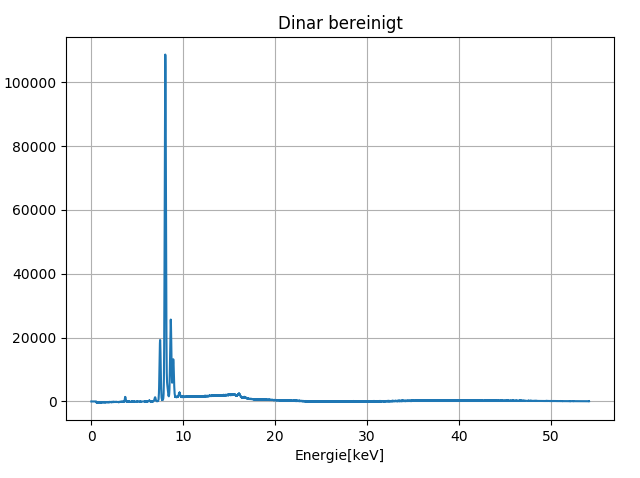
\includegraphics[scale=0.49]{Bilder/roentgen_spektren/dinar_0.png}
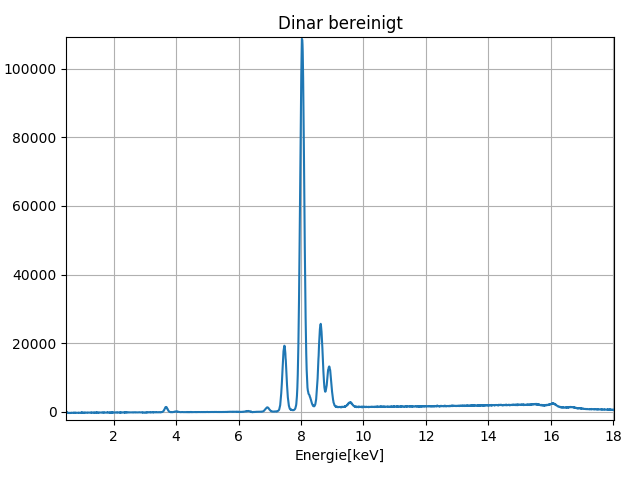
\includegraphics[scale=0.49]{Bilder/roentgen_spektren/dinar_1.png}
\caption{Von der Leermessung bereinigtes Spektrum des \textbf{Dinars} und zoom in den relevanten Bereich.}
\label{fig:prop_dinar}
\end{figure}
\begin{table}[H]
\center
\begin{tabular}{|c|c|c|c|c|}
\hline 
Peakpos.[keV] & Stoff & Linie & Literaturwert[keV] & Anmerkung \\
\hline 
$6.294 \pm 0.018 \pm 0.006$& $^{65}Tb$ & $L_{\alpha_{1/2}}$ & $6,238-6,272$ & \\
\hline 
$6.922 \pm 0.003 \pm 0.006$ & $^{27}Co$ & $K_{\alpha_{1/2}}$ & $6,915-6,930$ & \\ 
\hline 
$7.476 \pm 0.017 \pm 0.006$ & $^{28}Ni$ & $K_{\alpha_{1/2}}$ & $7,460-7,478$ & \\
\hline
$8.051 \pm 0.007 \pm 0.006$ & $^{29}Cu$ & $K_{\alpha_{1/2}}$ & $8,027-8,047$ & \\
\hline
$8.629 \pm 0.001 \pm 0.007$ & $^{30}Zn$ & $K_{\alpha_{1/2}}$ & $8,615-8,638$ & \\
\hline
$8.899 \pm 0.004 \pm 0.007$ & $^{29}Cu$ & $K_{\beta_{1/3}}$ & $8,905$ & \\
\hline
$9.570 \pm 0.001 \pm 0.007$ & $^{30}Zn$ & $K_{\beta_{1/3}}$ & $9,572$ & \\
\hline
$16.036 \pm 0.037 \pm 0.008$ & $^{38}Sr$ & $K_{\beta_{1/2/3}}$ & $15,824-16,084$ & \\
\hline
\end{tabular} 
\caption{Peaks in der Messung des Dinars}
\label{prop_dinar}
\end{table}

\newpage
\subsubsection{Pfennig}
\begin{figure}[H]
\centering
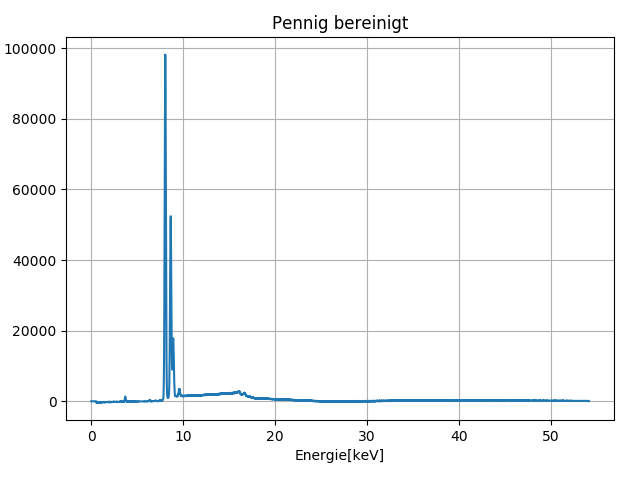
\includegraphics[scale=0.49]{Bilder/roentgen_spektren/pfennig_0.png}
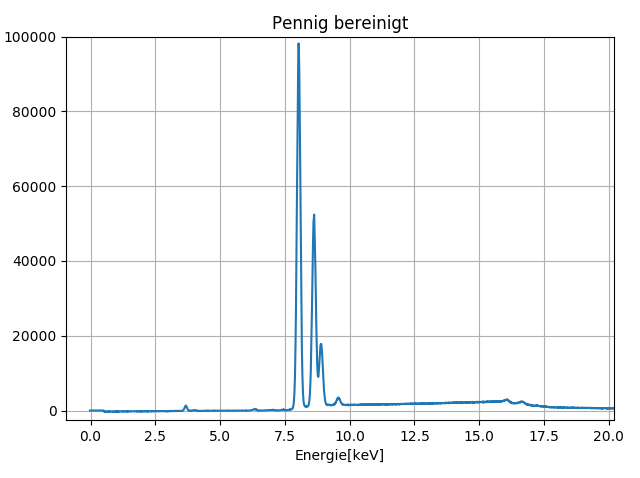
\includegraphics[scale=0.49]{Bilder/roentgen_spektren/pfennig_1.png}
\caption{Von der Leermessung bereinigtes Spektrum des \textbf{Pfennigs} und zoom in den relevanten Bereich.}
\label{fig:prop_dinar}
\end{figure}

\begin{table}[H]
\center
\begin{tabular}{|c|c|c|c|c|}
\hline 
Peakpos.[keV] & Stoff & Linie & Literaturwert[keV] & Anmerkung \\
\hline 
$6.329 \pm 0.01 \pm 0.006$& $^{65}Tb$ & $L_{\alpha_{1/2}}$ & $6,238-6,272$ & \\
& $^{26}De$ & $K_{\alpha_{1/2}}$ & $6,390-6,403$ & plausiebler\\
\hline 
$6.994 \pm 0.022 \pm 0.006$ & $^{27}Co$ & $K_{\alpha_{1/2}}$ & $6,915-6,930$ & \\ 
\hline 
$7.428 \pm 0.001 \pm 0.006$ & $^{28}Ni$ & $K_{\alpha_{1/2}}$ & $7,460-7,478$ & \\
\hline
$8.049 \pm 0.007 \pm 0.006$ & $^{29}Cu$ & $K_{\alpha_{1/2}}$ & $8,027-8,047$ & \\
\hline
$8.623 \pm 0.001 \pm 0.007$ & $^{30}Zn$ & $K_{\alpha_{1/2}}$ & $8,615-8,638$ & \\
\hline
$8.888 \pm 0.013 \pm 0.007$ & $^{29}Cu$ & $K_{\beta_{1/3}}$ & $8,905$ & \\
\hline
$9.563 \pm 0.001 \pm 0.007$ & $^{30}Zn$ & $K_{\beta_{1/3}}$ & $9,572$ & \\
\hline
$16.030 \pm 0.037 \pm 0.008$ & $^{38}Sr$ & $K_{\beta_{1/2/3}}$ & $15,824-16,084$ & \\
\hline
$16.639 \pm 0.033 \pm 0.008$ & $^{41}Nb$ & $K_{\alpha_{1/2}}$ & $16,521-16,615$ & \\
& $^{39}Y$ & $K_{\beta_{1/2/3}}$ & $16,725-16,737$ & \\
\hline
\end{tabular} 
\caption{Peaks in der Messung des Pfennigs}
\label{a_peaks_leer}
\end{table}

\newpage
\subsubsection{Rubel}
\begin{figure}[H]
\centering
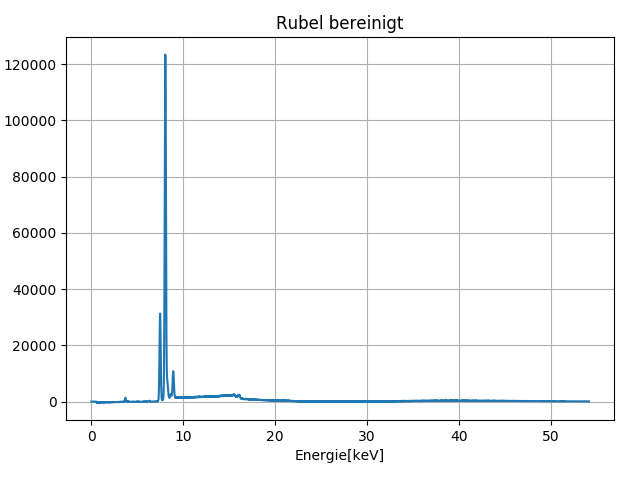
\includegraphics[scale=0.49]{Bilder/roentgen_spektren/rub_0.png}
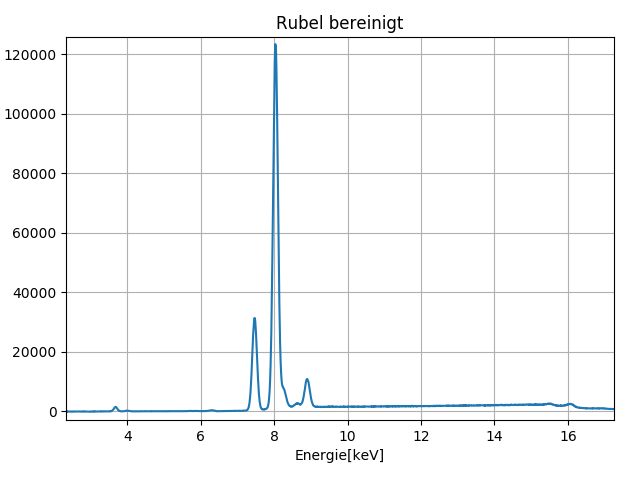
\includegraphics[scale=0.49]{Bilder/roentgen_spektren/rub_1.png}
\caption{Von der Leermessung bereinigtes Spektrum des \textbf{Rubels} und zoom in den relevanten Bereich.}
\label{fig:prop_rubel}
\end{figure}
\begin{table}[H]
\center
\begin{tabular}{|c|c|c|c|c|}
\hline 
Peakpos.[keV] & Stoff & Linie & Literaturwert[keV] & Anmerkung \\
\hline 
$6.296 \pm 0.008 \pm 0.006$& $^{65}Tb$ & $L_{\alpha_{1/2}}$ & $6,238-6,272$ & \\
\hline 
$7.465 \pm 0.004 \pm 0.006$ & $^{28}Ni$ & $K_{\alpha_{1/2}}$ & $7,460-7,478$ & \\
\hline
$8.050 \pm 0.012 \pm 0.006$ & $^{29}Cu$ & $K_{\alpha_{1/2}}$ & $8,027-8,047$ & \\
\hline
$8.644 \pm 0.013 \pm 0.007$ & $^{30}Zn$ & $K_{\alpha_{1/2}}$ & $8,615-8,638$ & \\
\hline
$8.899 \pm 0.001 \pm 0.007$ & $^{29}Cu$ & $K_{\beta_{1/3}}$ & $8,905$ & \\
\hline
$15.467 \pm 0.041 \pm 0.007$ & $^{30}Zn$ & $K_{\beta_{1/3}}$ & $9,572$ & \\
\hline
$16.032 \pm 0.046 \pm 0.008$ & $^{38}Sr$ & $K_{\beta_{1/2/3}}$ & $15,824-16,084$ & \\
\hline
\end{tabular} 
\caption{Peaks in der Messung des Rubels}
\label{prop_rubel}
\end{table}

\newpage
\subsubsection{Vergleich mit Erwartungen}
\paragraph{Stahl}
Das Spektrum von Stahl weißt die bereits gefundenen Linien wieder auf. Außerdem konnte der Inhalt von Eisen und Nickel bestätigt werden. Nickel ist ebenfalls ein oft für Legierungen verwendeter Stoff \footnote{\url{http://www.chemie.de/lexikon/Nickel.html}}, deswegen ist das Auftreten nicht verwunderlich.

\paragraph{Bleiblock}
Im Bleiblock konnten mehrere Linien von Blei endeckt werden. Diese haben auch die größte Intensität. Es wurde außerdem noch Antimon (Sb) gefunden. Dieses wird in Bleilegierungen verwendet\footnote{\url{https://de.wikipedia.org/wiki/Antimon}}.

\paragraph{Computerchip}
Im Prozessorchip wurden sehr viele unterschiedliche Stoffe gefunden, was auch zu erwarten war. Vor allem Molybdän sticht mit sehr hohen Intnsitäten heraus. Dises wird in Transistoren verwendet\footnote{\url{https://de.wikipedia.org/wiki/Molybdän}}, das Auftreten ist also vorrauszusehen. Auch Zinn und in sehr kleinen Mengen Gold wird in Chips verwendethttps:\footnote{\url{https://de.wikipedia.org/wiki/Zinn}}, der relativ hohe Zinnpeak kann also auch erklärt werden, sowie das Auftreten von Gold in einem kleinen Peak. Eisen und Wolfram sind gewöhnliche Stoffe für den Bau von Halterungen.

\paragraph{Magnet}
Von den gefundenen Stoffen ist nur Eisen und Dysprosium ferromagnetisch. \footnote{\url{https://de.wikipedia.org/wiki/Ferromagnetismus}}. Alle anderen Stoffe sind offensichtlich nur Teil der Legierung.

\paragraph{2 Dinara}
Diese Münze besteht aus Cu-Ni-Zn\footnote{\url{https://colnect.com/de/coins/coin/7997-2_Dinara-1963-1992_Sozialistische_Bundesrepublik_Jugoslawien-Jugoslawien}}. Alle Stoffe wurden im Spektrum gefunden, wobei der Kupferanteil am größten ist.

\paragraph{10 Pfennig}
Diese Münze besteht aus Fe-Cu-Zn\footnote{\url{https://colnect.com/de/coins/coin/840-10_Pfennig_A_D_F_G_J-1950~2001_DM_UmlaufmC3BCnzen-Deutschland_BRD}}. Dabei ist Eisen der größte Peak. Auch hier konnten alle drei Stoffe identifiziert werden.

\paragraph{10 Rubel}
Es ist nicht genau klar, welche Art von Rubel diese Münze war. Allerdings wird aus dem gefundenen Spektrum auf eine Kupfer-Zink-Nickel Legierung geschlossen.


\subsection{Energieauflösung}

\section{Fazit}
\section{Anhang}
\subsection{Kalibration $\alpha$-Quelle}
\begin{figure}[H]
\centering
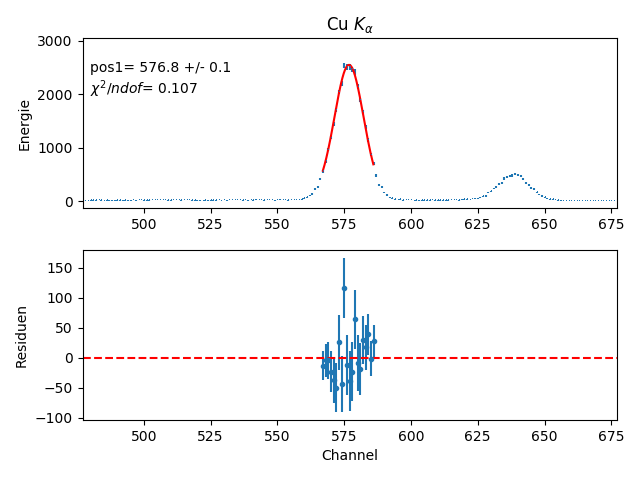
\includegraphics[scale=0.8]{Bilder/alpha/cu_alpha_1.png}
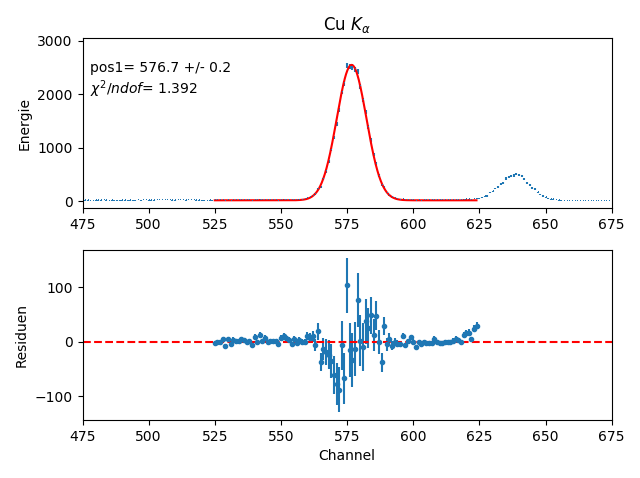
\includegraphics[scale=0.8]{Bilder/alpha/cu_alpha_2.png}
\caption{Alle für dei Kalibration aufgenommenen Spektren.}
\label{fig:kal_alles}
\end{figure}
\begin{figure}[H]
\centering
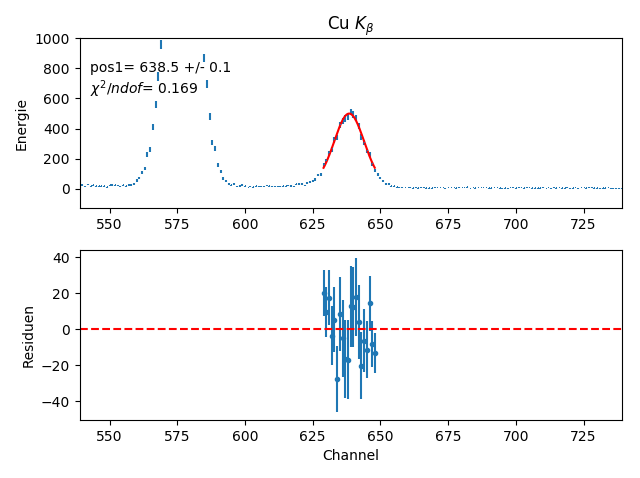
\includegraphics[scale=0.8]{Bilder/alpha/cu_beta_1.png}
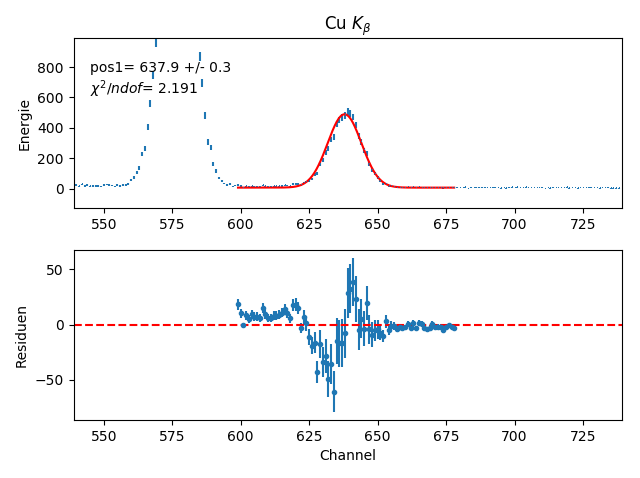
\includegraphics[scale=0.8]{Bilder/alpha/cu_beta_2.png}
\caption{Alle für dei Kalibration aufgenommenen Spektren.}
\label{fig:kal_alles}
\end{figure}

\begin{figure}[H]
\centering
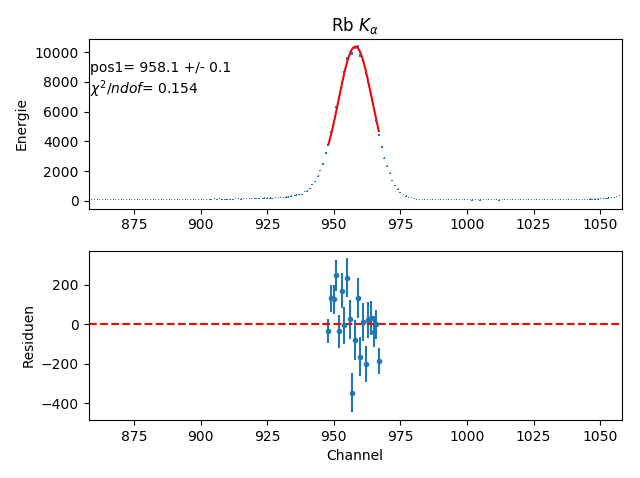
\includegraphics[scale=0.8]{Bilder/alpha/rb_alpha_1.png}
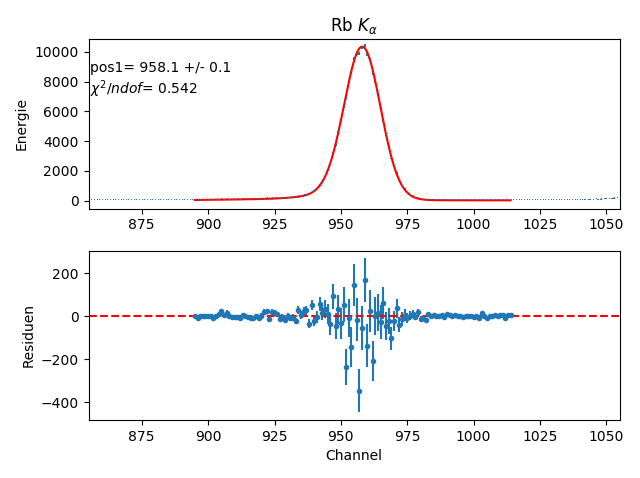
\includegraphics[scale=0.8]{Bilder/alpha/rb_alpha_2.png}
\caption{Alle für dei Kalibration aufgenommenen Spektren.}
\label{fig:kal_alles}
\end{figure}
\begin{figure}[H]
\centering
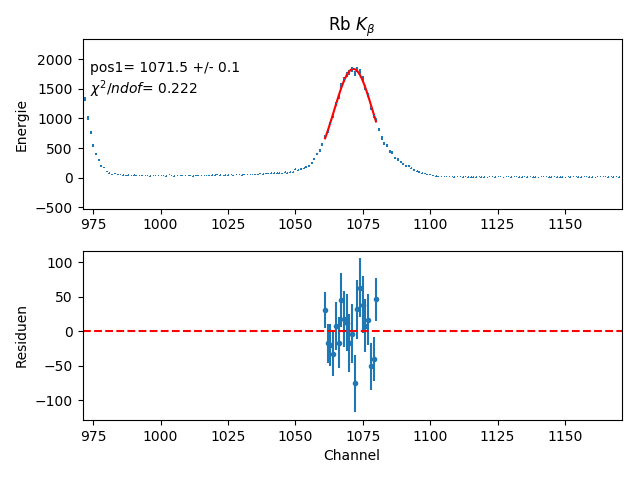
\includegraphics[scale=0.8]{Bilder/alpha/rb_beta_1.png}
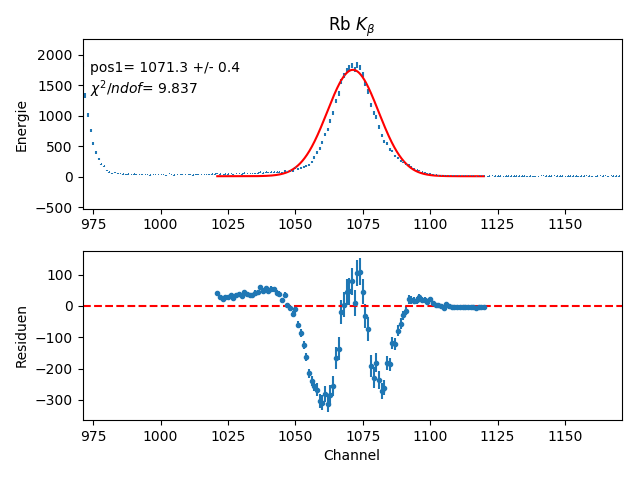
\includegraphics[scale=0.8]{Bilder/alpha/rb_beta_2.png}
\caption{Alle für dei Kalibration aufgenommenen Spektren.}
\label{fig:kal_alles}
\end{figure}

\begin{figure}[H]
\centering
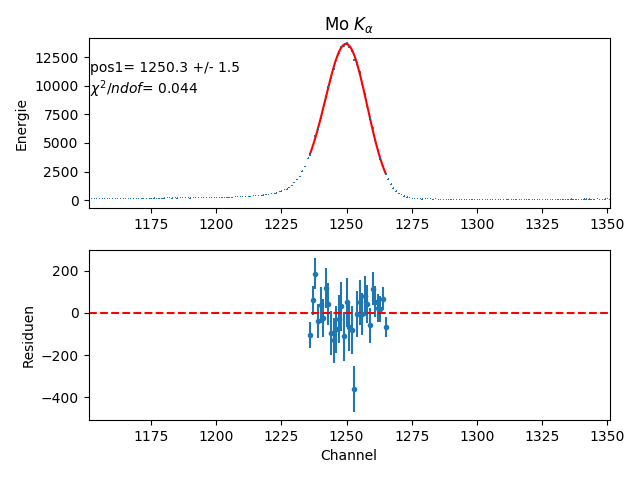
\includegraphics[scale=0.8]{Bilder/alpha/mo_alpha_1.png}
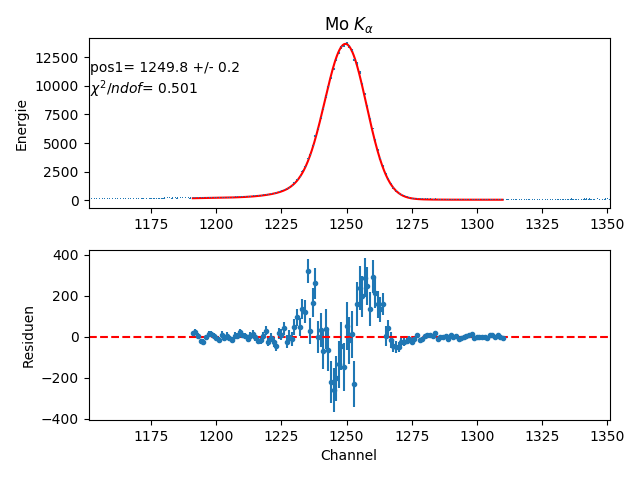
\includegraphics[scale=0.8]{Bilder/alpha/mo_alpha_2.png}
\caption{Alle für dei Kalibration aufgenommenen Spektren.}
\label{fig:kal_alles}
\end{figure}
\begin{figure}[H]
\centering
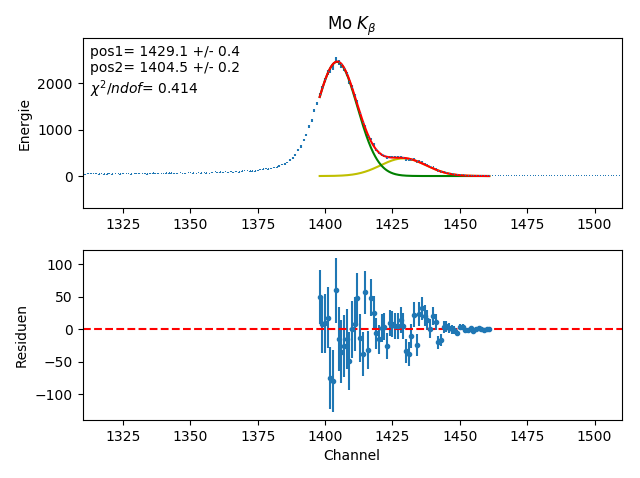
\includegraphics[scale=0.8]{Bilder/alpha/mo_beta_1.png}
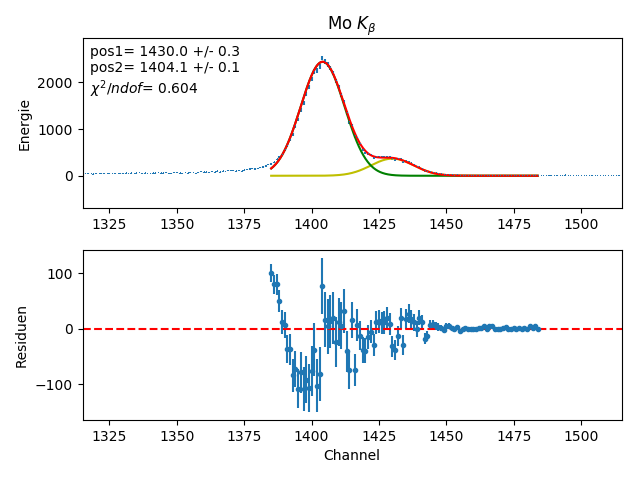
\includegraphics[scale=0.8]{Bilder/alpha/mo_beta_2.png}
\caption{Alle für dei Kalibration aufgenommenen Spektren.}
\label{fig:kal_alles}
\end{figure}

\begin{figure}[H]
\centering
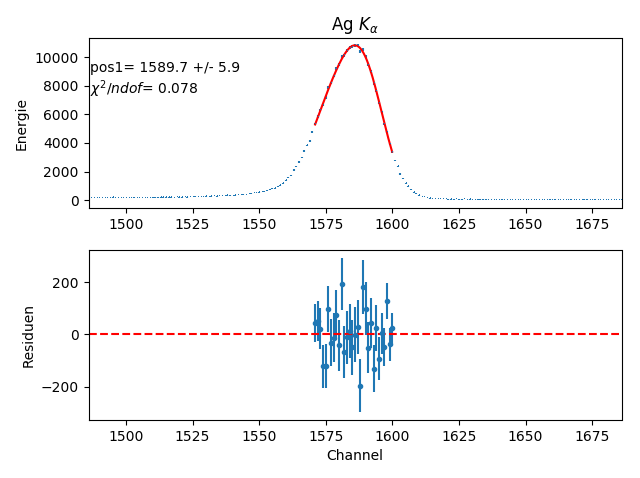
\includegraphics[scale=0.8]{Bilder/alpha/ag_alpha_1.png}
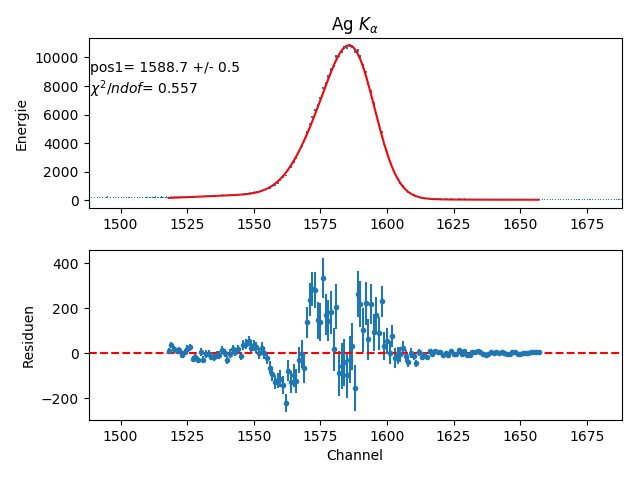
\includegraphics[scale=0.8]{Bilder/alpha/ag_alpha_2.png}
\caption{Alle für dei Kalibration aufgenommenen Spektren.}
\label{fig:kal_alles}
\end{figure}
\begin{figure}[H]
\centering
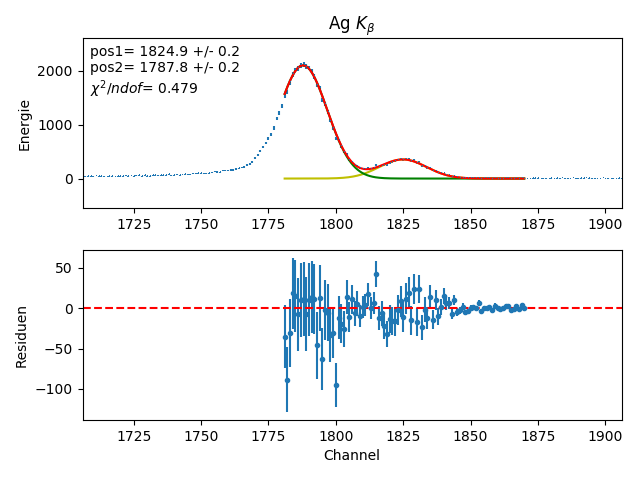
\includegraphics[scale=0.8]{Bilder/alpha/ag_beta_1.png}
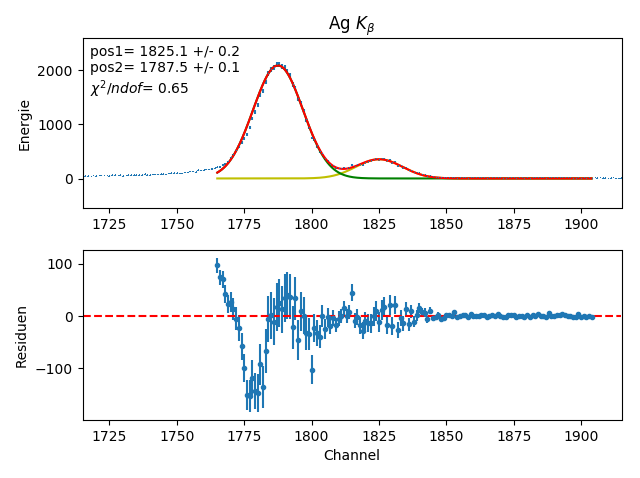
\includegraphics[scale=0.8]{Bilder/alpha/ag_beta_2.png}
\caption{Alle für dei Kalibration aufgenommenen Spektren.}
\label{fig:kal_alles}
\end{figure}

\begin{figure}[H]
\centering
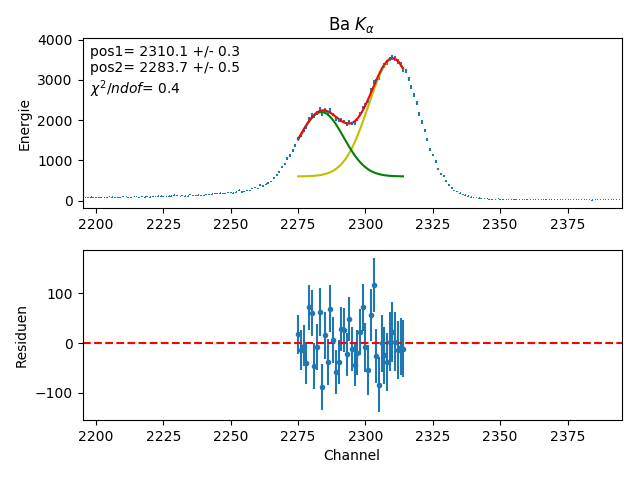
\includegraphics[scale=0.8]{Bilder/alpha/ba_alpha_1.png}
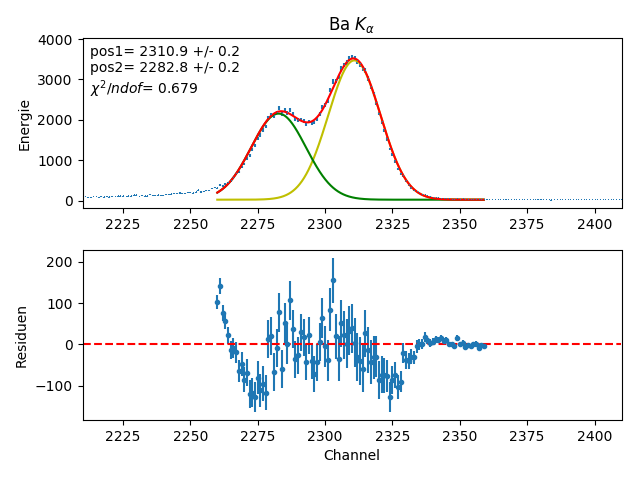
\includegraphics[scale=0.8]{Bilder/alpha/ba_alpha_2.png}
\caption{Alle für dei Kalibration aufgenommenen Spektren.}
\label{fig:kal_alles}
\end{figure}
\begin{figure}[H]
\centering
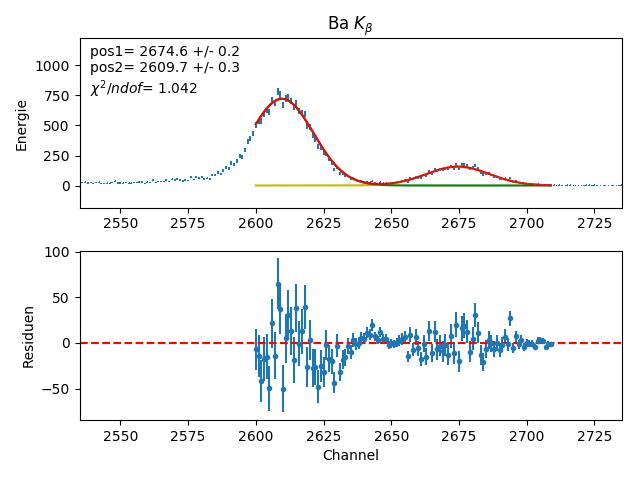
\includegraphics[scale=0.8]{Bilder/alpha/ba_beta_1.png}
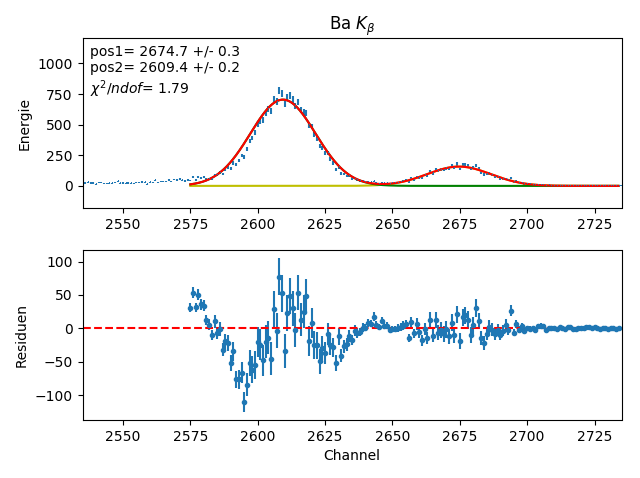
\includegraphics[scale=0.8]{Bilder/alpha/ba_beta_2.png}
\caption{Alle für dei Kalibration aufgenommenen Spektren.}
\label{fig:kal_alles}
\end{figure}

\begin{figure}[H]
\centering
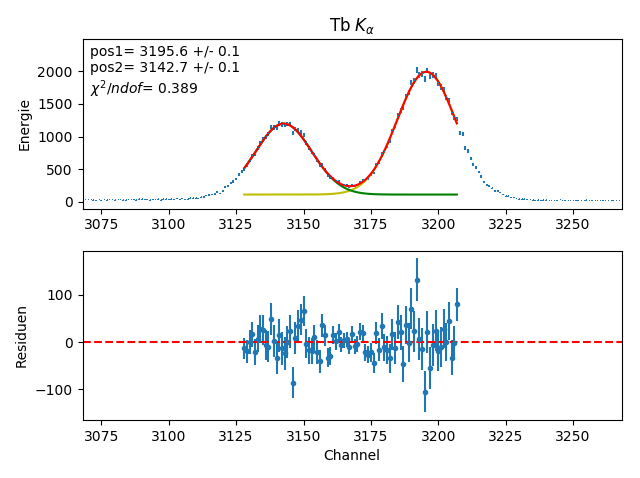
\includegraphics[scale=0.8]{Bilder/alpha/tb_alpha_1.png}
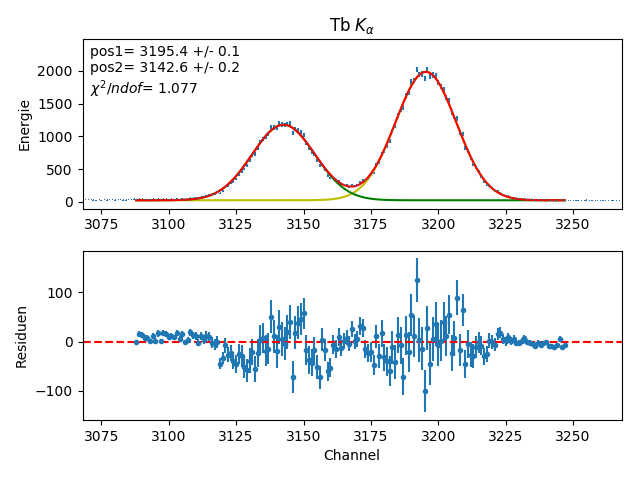
\includegraphics[scale=0.8]{Bilder/alpha/tb_alpha_2.png}
\caption{Alle für dei Kalibration aufgenommenen Spektren.}
\label{fig:kal_alles}
\end{figure}
\begin{figure}[H]
\centering
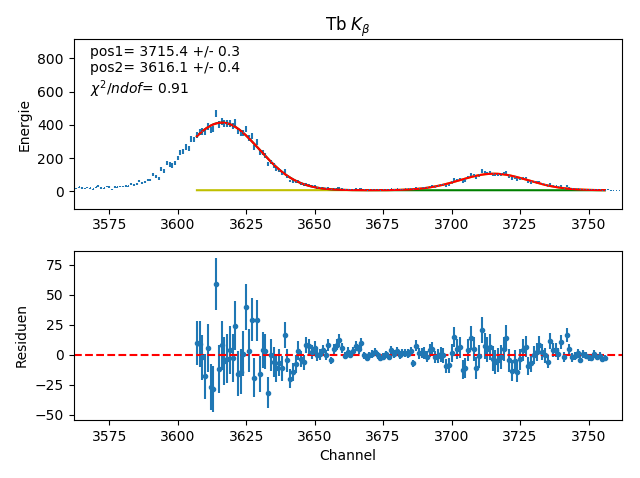
\includegraphics[scale=0.8]{Bilder/alpha/tb_beta_1.png}
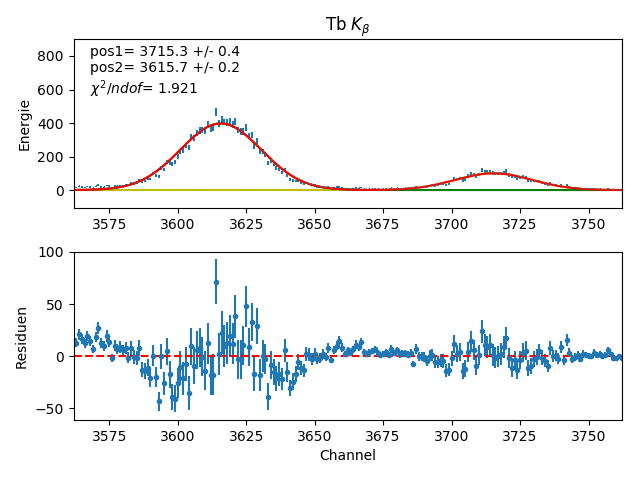
\includegraphics[scale=0.8]{Bilder/alpha/tb_beta_2.png}
\caption{Alle für dei Kalibration aufgenommenen Spektren.}
\label{fig:kal_alles}
\end{figure}
\subsection{unbekannte Proben $\alpha$-Quelle}
\subsubsection{Leermessung}
\begin{figure}[H]
\centering
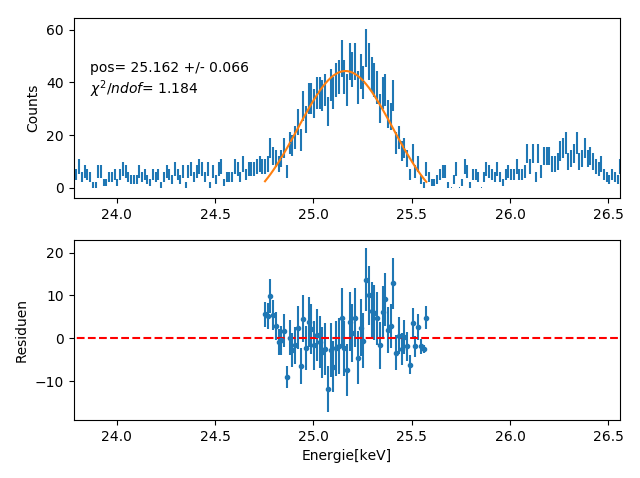
\includegraphics[scale=0.49]{Bilder/alpha_spektren/leer_1_1.png}
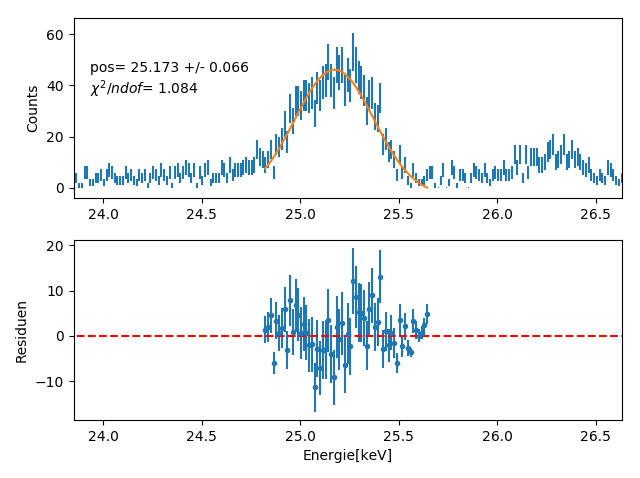
\includegraphics[scale=0.49]{Bilder/alpha_spektren/leer_1_2.png}
\caption{Leermessung Peak1}
\end{figure}
\begin{figure}[H]
\centering
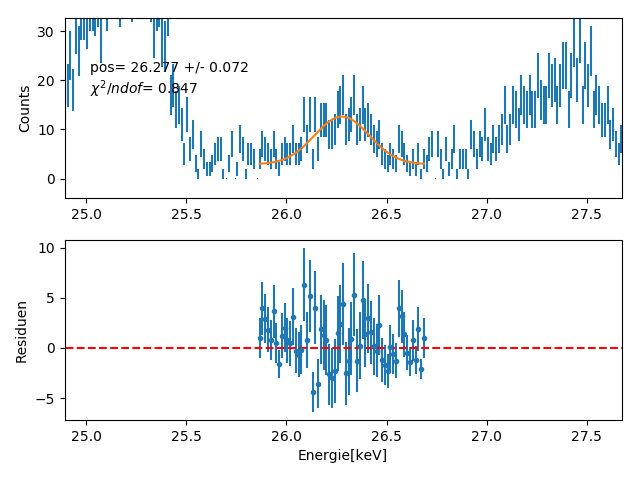
\includegraphics[scale=0.49]{Bilder/alpha_spektren/leer_2_1.png}
\includegraphics[scale=0.49]{Bilder/alpha_spektren/leer_2_2.png}
\caption{Leermessung Peak2}
\end{figure}
\begin{figure}[H]
\centering
\includegraphics[scale=0.49]{Bilder/alpha_spektren/leer_3_1.png}
\includegraphics[scale=0.49]{Bilder/alpha_spektren/leer_3_2.png}
\caption{Leermessung Peak3}
\end{figure}

\begin{figure}[H]
\centering
\includegraphics[scale=0.49]{Bilder/alpha_spektren/leer_4_1.png}
\includegraphics[scale=0.49]{Bilder/alpha_spektren/leer_4_2.png}
\caption{Leermessung Peak4}
\end{figure}

\begin{figure}[H]
\centering
\includegraphics[scale=0.49]{Bilder/alpha_spektren/leer_5_1.png}
\includegraphics[scale=0.49]{Bilder/alpha_spektren/leer_5_2.png}
\caption{Leermessung Peak5}
\end{figure}

\begin{figure}[H]
\centering
\includegraphics[scale=0.49]{Bilder/alpha_spektren/leer_6_1.png}
\includegraphics[scale=0.49]{Bilder/alpha_spektren/leer_6_2.png}
\caption{Leermessung Peak6}
\end{figure}
\subsubsection{Stahl}
\begin{figure}[H]
\centering
\includegraphics[scale=0.49]{Bilder/alpha_spektren/stahl_1_1.png}
\includegraphics[scale=0.49]{Bilder/alpha_spektren/stahl_1_2.png}
\caption{Stahl Peak6}
\end{figure}
\begin{figure}[H]
\centering
\includegraphics[scale=0.49]{Bilder/alpha_spektren/stahl_2_1.png}
\includegraphics[scale=0.49]{Bilder/alpha_spektren/stahl_2_2.png}
\caption{Stahl Peak2}
\end{figure}
\begin{figure}[H]
\centering
\includegraphics[scale=0.49]{Bilder/alpha_spektren/stahl_3_1.png}
\includegraphics[scale=0.49]{Bilder/alpha_spektren/stahl_3_2.png}
\caption{Stahl Peak3}
\end{figure}

\end{document}
